\pagestyle{fancy}
\fancyhead[LO]{\autorR}
\fancyhead[LE]{\autorA}
\fancyhead[RE,RO]{\textit{\rightmark}}
\fancyfoot[L]{\asignaturaAbbr}
\fancyfoot[R]{\fecha}

\section{Equations}
\label{sec:Equations}

\subsection{Problema a resolver}

El problema consiste en la resolución de un sistema de ecuaciones lineales
(SEL) de un tamaño cualquiera mediante el método de Gauss-Jordan.
Para ello, se recibe como dato de entrada el tamaño del SEL
(i.e. su número de incógnitas).
De esta forma, un problema $N=3$ sería de la forma representada en la
ecuación \ref{eq:sel}.

\begin{mycapequ}[h]
\begin{equation}
\begin{matrix}
    a_{0,0} \cdot x_0 & + & a_{0,1} \cdot x_1 & + & a_{0,2} \cdot x_2 & = & y_0 \\
    a_{1,0} \cdot x_0 & + & a_{1,1} \cdot x_1 & + & a_{1,2} \cdot x_2 & = & y_1 \\
    a_{2,0} \cdot x_0 & + & a_{2,1} \cdot x_1 & + & a_{2,2} \cdot x_2 & = & y_2
\end{matrix}
\end{equation}
\caption{Sistema de ecuaciones lineales (SEL)}
\label{eq:sel}
\end{mycapequ}

Se utiliza como dato de entrada una matriz de tamaño $N \times N+1$.
Esta estructura contiene los $N$ coeficientes del SEL en sus primeras $N$
columnas y el vector de términos independientes en la columna $N+1$.
(Véase \ref{eq:sel_matrix})

\begin{mycapequ}[h]
\begin{equation}
    \begin{bmatrix}
        a_{0,0} & a_{0,1} & a_{0,2} & \cdots & a_{0,N} & y_0 \\
        a_{1,0} & a_{1,1} & a_{1,2} & \cdots & a_{1,N} & y_1 \\
        \vdots & \vdots & \vdots & \ddots & \vdots & \vdots \\
        a_{N,0} & a_{N,1} & a_{N,2} & \cdots & a_{N,N} & y_N \\
    \end{bmatrix}
\end{equation}
\caption{Matriz de coeficientes extendida de un SEL}
\label{eq:sel_matrix}
\end{mycapequ}

A esta matriz se le aplicarán una serie de transformaciones según el método
de Gauss Jordan para obtener una matriz identidad,
en la que su diagonal principal está compuesta de unos y el resto de elementos
son cero (salvo los términos independientes de la columna $N+1$).
Estos términos independientes serán el resultado del SEL.
Esta matriz sería de la forma:

\begin{mycapequ}[h]
\begin{equation}
    \begin{bmatrix}
        1 & 0 & 0 & \cdots & 0 & x_0 \\
        0 & 1 & 0 & \cdots & 0 & x_1 \\
        0 & 0 & 1 & \cdots & 0 & x_2 \\
        \vdots & \vdots & \vdots & \ddots & \vdots & \vdots \\
        0 & 0 & 0 & \cdots & 1 & x_N
    \end{bmatrix}
\end{equation}
\caption{Matriz identidad de un sistema de ecuaciones lineales}
\label{eq:sel_identity}
\end{mycapequ}

\subsection{CPU}

Las observacinoes empíricas del algoritmo en CPU siguen fielmente
las predicciones teóricas para este algoritmo.
Se presenta una gráfica que muestra el comportamiento potencial
del tiempo de ejecución respecto al tamaño del problema.
Nótese que ambos ejes de la gráfica son logarítmicos.
Véase \ref{fig:gpu_time}.

\subsection{GPU}

La aceleración de un algoritmo paralelo se decide
en el instante en que se planifican las secciones paralelas,
sus tareas, comunicaciones, sincronización y dependencias.
En el caso de Gauss Jordan, paralelizar el computo
de cada columna es inviable, ya que cada columna
depende de la columna anterior.
En su lugar, se debe dividir el cómputo de cada columna
en dos partes paralelas: en la primera se normaliza la fila
para obtener el 1 en la diagonal principal
(\texttt{normalize\_row}),
y en la segunda se obtienen ceros en la columna actual
(\texttt{eliminate\_column}).
Este acercamiento reporta una tiempo notablemente mejor
al de la CPU. Véase \ref{fig:gpu_time}

\begin{figure}[h]
    \centering
    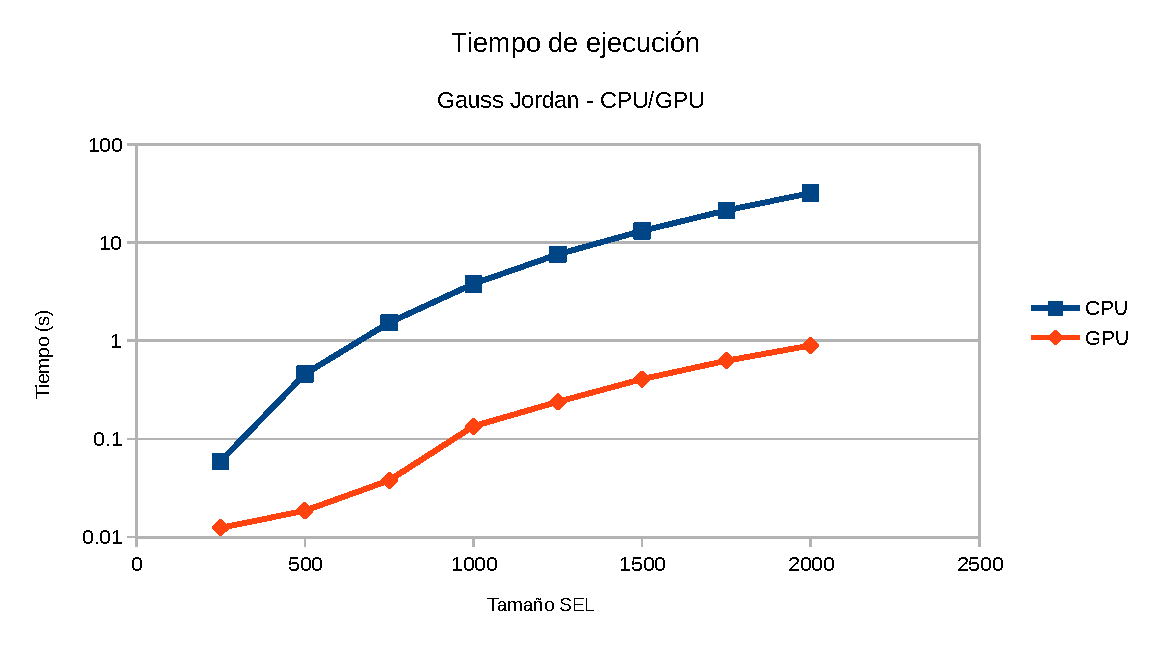
\includegraphics[width=0.7\textwidth]{img/EQ_GPU_TIME.pdf}
    \caption{Tiempos de ejecución de para varios tamaños.}
    \label{fig:gpu_time}
\end{figure}

Debido al gran tamaño de las matrices probadas,
en las que se exceden los 1024 elementos por fila y columna,
se han utilizado varios bloques de hilos,
calculados dinámicamente en tiempo de ejecución
a partir del tamaño de la matriz.
En todos los casos, el tamaño de la matriz se reparte entre bloques
del máximo tamaño posible.
De los dos kernels utilizados, 
el primero (\texttt{normalize\_row})
utiliza una estructura unidimensional de hilos y bloques
para iterar por todas las columnas de una fila
de la matriz.
El segundo (\texttt{eliminate\_column})
utiliza una estructura bidimensional de hilos y bloques
para iterar por todas las columnas y filas de la matriz,
anulando la columna actual y aplicando el mismo
factor al resto de columnas de la fila.
Véase \ref{fig:KernelsGaussJordanGPU}.

\begin{figure}[h]
\centering
\begin{subfigure}[b]{0.45\textwidth}
\centering
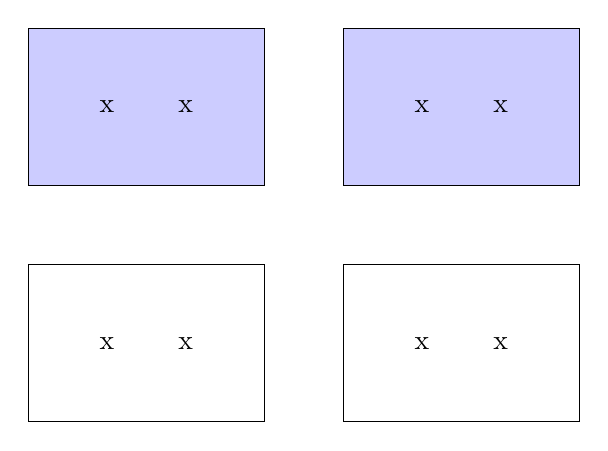
\begin{tikzpicture}
    \draw [rectangle, fill=blue!20] (0,0) rectangle (3,2);
    \node at (1,1) {x};
    \node at (2,1) {x};
    \draw [rectangle, fill=blue!20] (4,0) rectangle (7,2);
    \node at (5,1) {x};
    \node at (6,1) {x};

    \draw [rectangle] (0,-1) rectangle (3,-3);
    \node at (1,-2) {x};
    \node at (2,-2) {x};
    \draw [rectangle] (4,-1) rectangle (7,-3);
    \node at (5,-2) {x};
    \node at (6,-2) {x};
\end{tikzpicture}
\caption{Kernel \texttt{normalize\_row}}
\end{subfigure}
\hfill
\begin{subfigure}[b]{0.45\textwidth}
\centering
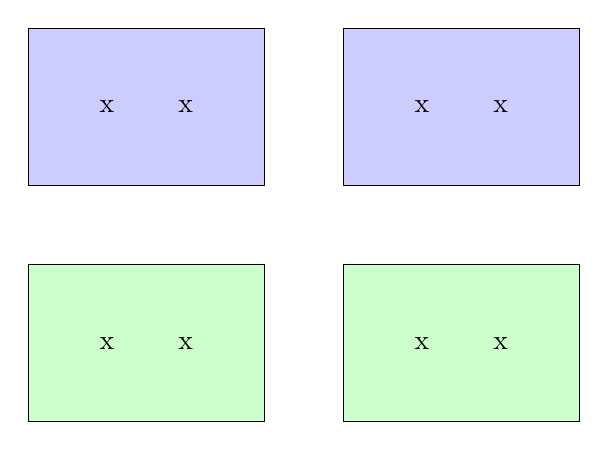
\begin{tikzpicture}
    \draw [rectangle, fill=blue!20] (0,0) rectangle (3,2);
    \node at (1,1) {x};
    \node at (2,1) {x};
    \draw [rectangle, fill=blue!20] (4,0) rectangle (7,2);
    \node at (5,1) {x};
    \node at (6,1) {x};

    \draw [rectangle, fill=green!20] (0,-1) rectangle (3,-3);
    \node at (1,-2) {x};
    \node at (2,-2) {x};
    \draw [rectangle, fill=green!20] (4,-1) rectangle (7,-3);
    \node at (5,-2) {x};
    \node at (6,-2) {x};
\end{tikzpicture}
\caption{Kernel \texttt{eliminate\_column}}
\end{subfigure}
\caption{Kernels de Gauss Jordan en GPU}
\label{fig:KernelsGaussJordanGPU}
\end{figure}

\pagebreak
Siguiendo este sistema,
el trabajo realizado por los hilos
para cada columna se representa
con el diagrama \ref{fig:GaussJordanGPU}.
Se pueden ver dos puntos de sincronización
en los que el paralelismo se rompe (nodos azules),
el kernel \texttt{normalize\_row} que se ejecuta sobre
el número de filas (nodos verdes)
y el kernel \texttt{eliminate\_column} que se ejecuta sobre
el número total de celdas (nodos rojos).

\begin{figure}[h]
\centering
\resizebox{.9375\linewidth}{!}{
\begin{tikzpicture}
    \draw [circle, fill=blue!20] (0,0) circle (1);

    \draw [circle, fill=green!20] (3,1) circle (1);
    \draw [circle, fill=green!20] (3,-1) circle (1);
    \draw [circle, fill=green!20] (3,3) circle (1);
    \draw [circle, fill=green!20] (3,-3) circle (1);

    \draw [circle, fill=blue!20] (6,0) circle (1);

    \draw [circle, fill=red!20] (10,-7.5) circle (1);
    \draw [circle, fill=red!20] (10,-6.5) circle (1);
    \draw [circle, fill=red!20] (10,-5.5) circle (1);
    \draw [circle, fill=red!20] (10,-4.5) circle (1);
    \draw [circle, fill=red!20] (10,-3.5) circle (1);
    \draw [circle, fill=red!20] (10,-2.5) circle (1);
    \draw [circle, fill=red!20] (10,-1.5) circle (1);
    \draw [circle, fill=red!20] (10,-0.5) circle (1);
    \draw [circle, fill=red!20] (10,0.5) circle (1);
    \draw [circle, fill=red!20] (10,1.5) circle (1);
    \draw [circle, fill=red!20] (10,2.5) circle (1);
    \draw [circle, fill=red!20] (10,3.5) circle (1);
    \draw [circle, fill=red!20] (10,4.5) circle (1);
    \draw [circle, fill=red!20] (10,5.5) circle (1);
    \draw [circle, fill=red!20] (10,6.5) circle (1);
    \draw [circle, fill=red!20] (10,7.5) circle (1);

    \draw [circle, fill=blue!20] (15,0) circle (1);

    \draw [arrow] (1,0) -- (2,1);
    \draw [arrow] (1,0) -- (2,-1);
    \draw [arrow] (1,0) -- (2,3);
    \draw [arrow] (1,0) -- (2,-3);

    \draw [arrow] (4,1) -- (5, 0);
    \draw [arrow] (4,-1) -- (5, 0);
    \draw [arrow] (4,3) -- (5, 0);
    \draw [arrow] (4,-3) -- (5, 0);

    \draw [arrow] (7,0) -- (9,0.5);
    \draw [arrow] (7,0) -- (9,-0.5);
    \draw [arrow] (7,0) -- (9,1.5);
    \draw [arrow] (7,0) -- (9,-1.5);
    \draw [arrow] (7,0) -- (9,2.5);
    \draw [arrow] (7,0) -- (9,-2.5);
    \draw [arrow] (7,0) -- (9,3.5);
    \draw [arrow] (7,0) -- (9,-3.5);
    \draw [arrow] (7,0) -- (9,4.5);
    \draw [arrow] (7,0) -- (9,-4.5);
    \draw [arrow] (7,0) -- (9,5.5);
    \draw [arrow] (7,0) -- (9,-5.5);
    \draw [arrow] (7,0) -- (9,6.5);
    \draw [arrow] (7,0) -- (9,-6.5);
    \draw [arrow] (7,0) -- (9,7.5);
    \draw [arrow] (7,0) -- (9,-7.5);

    \draw [arrow] (11,0.5) -- (14, 0);
    \draw [arrow] (11,-0.5) -- (14, 0);
    \draw [arrow] (11,1.5) -- (14, 0);
    \draw [arrow] (11,-1.5) -- (14, 0);
    \draw [arrow] (11,2.5) -- (14, 0);
    \draw [arrow] (11,-2.5) -- (14, 0);
    \draw [arrow] (11,3.5) -- (14, 0);
    \draw [arrow] (11,-3.5) -- (14, 0);
    \draw [arrow] (11,4.5) -- (14, 0);
    \draw [arrow] (11,-4.5) -- (14, 0);
    \draw [arrow] (11,5.5) -- (14, 0);
    \draw [arrow] (11,-5.5) -- (14, 0);
    \draw [arrow] (11,6.5) -- (14, 0);
    \draw [arrow] (11,-6.5) -- (14, 0);
    \draw [arrow] (11,7.5) -- (14, 0);
    \draw [arrow] (11,-7.5) -- (14, 0);
\end{tikzpicture}
}
\caption{Cálculo de Gauss Jordan en GPU}
\label{fig:GaussJordanGPU}
\end{figure}
